Having in mind that the product we want to study is an item that generates interest in much more women than men we decided to focus our studies on only women. We also came to the conclusion that since a luxury scarf it's usually bought from the middle and the upper class a minimum family yearly income bound was necessary to set our focus on only the users that are able to generate more impact on the analysis. We set this bound at 80.000 \EUR{} gross. Finally we thought that since trends can vary among countries, considering only the Italian population was better.
The features that we decided to observe on our users are:
\begin{itemize}
	\item \textbf{With/Without children}:\@ To better observe the impact that a son can have in buying a luxury item
	\item \textbf{Living in the North/South of Italy}:\@ To better observe the impact that the climate can have in buying an item that is useful only in certain seasons.
\end{itemize}
The probabilities of these users are described in the following pie chart:
\makebox[\textwidth][c]{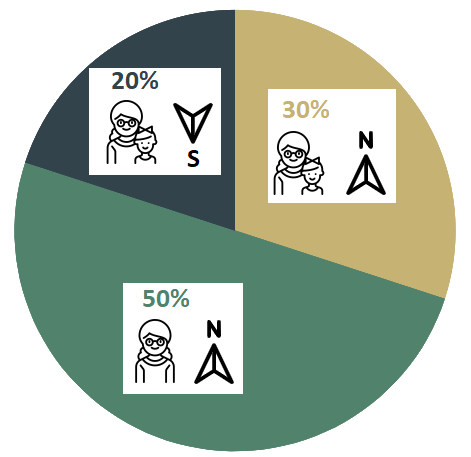
\includegraphics[width=0.7\textwidth]{sections/usersImage2}}
%\makebox[\textwidth][c]{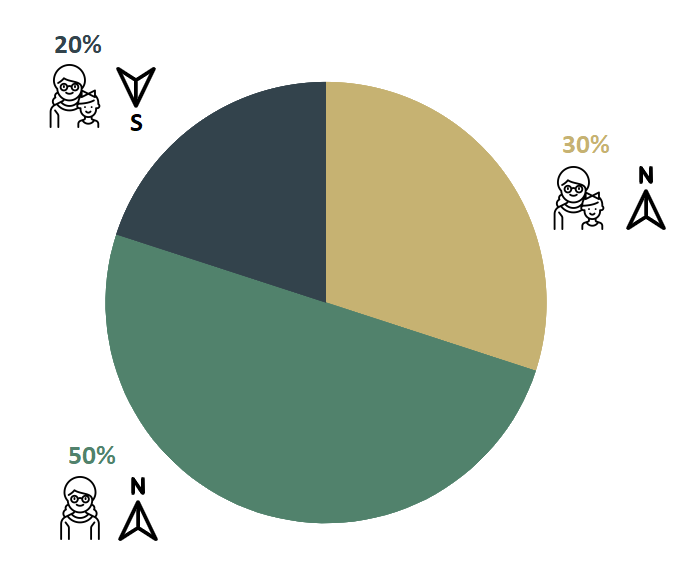
\includegraphics[width=0.9\textwidth]{sections/usersImage}}